\documentclass[twocolumn,10pt]{article}
\usepackage[utf8]{inputenc}
\usepackage[margin=0.75in]{geometry}
\usepackage{amsmath,amssymb}
\usepackage{graphicx}
\usepackage{booktabs}
\usepackage{microtype}
\usepackage{hyperref}
\usepackage{natbib}

\hypersetup{
    colorlinks=true,
    linkcolor=blue,
    citecolor=blue,
    urlcolor=blue
}

\title{\textbf{Coupled Hydrodynamic Envelope Stripping and Tidal Orbital Decay in Ultra-Short-Period Gas Giants}}
\author{\textbf{Antigravity Exoplanet Science Collaboration}}
\date{\today}

\begin{document}

\maketitle

\begin{abstract}
Ultra-Short-Period (USP) gas giant exoplanets ($a \lesssim 0.035\text{ AU}$, $P_{\text{orb}} \lesssim 2\text{ days}$) experience extreme tidal gravitational forces and intense stellar irradiation, bringing them near their volume-equivalent Roche lobe limits. Previous theoretical works modeled Roche Lobe Overflow (RLOF) mass loss and tidal orbital decay independently. In this study, we construct a fully coupled 1D hydrostatic and orbital evolution model that simultaneously solves for planetary interior thermal cooling ($\dot{S}_{\text{env}}$), hydrodynamic envelope stripping ($\dot{M}_{\text{RLOF}}$), and tidal semi-major axis decay ($\dot{a}_{\text{tide}}$). We explore a 4D simulation matrix across planetary masses ($0.4\text{--}2.0\,M_{\text{Jup}}$) and orbital separations ($0.015\text{--}0.035\text{ AU}$). We discover a fundamental non-linear bifurcation in planetary fate: (1) \textit{Tidal Runaway Disruption}, where envelope stripping accelerates inward orbital migration, causing total planetary engulfment within $\lesssim 1\text{ Gyr}$, and (2) \textit{Self-Limiting Mass-Loss Stagnation}, where envelope removal contracts the planetary radius ($R_p$), causing the planet to slip back inside its Roche lobe ($\mu_{\text{Roche}} < 1$) and survive as a stable USP gas giant or remnant core. We compare our empirical survival boundaries against the observed sample of 362 transiting gas giants from our relational database (\texttt{hot\_jupiter.db}), accurately reproducing the scarcity of low-mass giants at $a \le 0.02\text{ AU}$ and providing quantitative predictions for PLATO and Ariel.
\end{abstract}

\section{Introduction}
The discovery of transiting Ultra-Short-Period (USP) giant planets such as WASP-12b ($P_{\text{orb}} = 1.09\text{ d}$, $a = 0.0229\text{ AU}$), WASP-19b ($P_{\text{orb}} = 0.79\text{ d}$, $a = 0.0163\text{ AU}$), and NGTS-10b ($P_{\text{orb}} = 0.76\text{ d}$, $a = 0.0143\text{ AU}$) has challenged our understanding of planetary survival under extreme physical environments \citep{Charbonneau2000, Dawson2018}. Located at the extreme inner boundary of planetary orbital space, these gas giants are subject to intense tidal gravitational torques from their host stars and incident stellar flux exceeding $F_{\text{inc}} \gtrsim 10^6\text{ W m}^{-2}$.

When a planet's physical radius ($R_p$) approaches or exceeds its volume-equivalent Roche lobe radius ($R_{\text{Roche}}$), atmospheric gas flows through the inner Lagrange point ($L_1$), initiating Roche Lobe Overflow (RLOF) envelope stripping \citep{Eggleton1983, Li2010}. Simultaneously, tidal dissipation in the planetary interior dissipates orbital energy, driving orbital decay ($\left.da/dt\right|_{\text{tide}} < 0$) and depositing tidal power ($P_{\text{tidal}}$) into the planetary core and envelope \citep{Hut1981, Leconte2010}.

Historically, theoretical studies evaluated RLOF mass loss assuming fixed orbital separations \citep{Jackson2017} or modeled tidal circularization assuming static planetary radii \citep{Eggleton1998}. However, mass loss alters planetary mass ($M_p$) and orbital angular momentum ($\left.da/dt\right|_{\text{RLOF}}$), while tidal heating inflates the planetary envelope, altering the Roche lobe filling factor $\mu_{\text{Roche}} \equiv R_p / R_{\text{Roche}}$. 

In this paper, we present the first unified 1D hydrostatic and orbital evolutionary framework that couples time-dependent RLOF mass loss, tidal circularization, and interior structural thermodynamics.

\section{Coupled Numerical Framework}
We couple the 1D hydrostatic interior solver \texttt{InteriorSolver} from the \texttt{hot\_jupiter} numerical code with dynamic orbital and mass-loss differential equations.

\subsection{1D Hydrostatic Interior \& EOS}
The planetary interior envelope is integrated from the core-envelope boundary to the atmospheric surface under hydrostatic equilibrium:
\begin{equation}
\frac{dP}{dr} = -\frac{G M(r) \rho(r)}{r^2}, \quad \frac{dM}{dr} = 4\pi r^2 \rho(r)
\end{equation}
using the hydrogen-helium equation of state (EOS) \citep{Saumon1995, Chabrier2019}. The atmospheric boundary condition is governed by the double-gray radiative transfer profile \citep{Guillot2010}:
\begin{equation}
T^4(\tau) = \frac{3 T_{\text{int}}^4}{4} \left( \tau + \frac{2}{3} \right) + \frac{3 T_{\text{irr}}^4}{4} \mu_0 \left[ \frac{2}{3} + \frac{1}{\gamma\sqrt{3}} + \left( \frac{\gamma}{\sqrt{3}} - \frac{1}{\gamma\sqrt{3}} \right) e^{-\gamma \tau \sqrt{3}} \right]
\end{equation}
where $T_{\text{int}} = (L_{\text{int}} / 4\pi R_p^2 \sigma)^{1/4}$ is the intrinsic effective temperature.

\subsection{Hydrodynamic RLOF Mass Loss}
The volume-equivalent Roche lobe radius is calculated using the standard formulation \citep{Eggleton1983}:
\begin{equation}
R_{\text{Roche}} = a \frac{0.49 q^{2/3}}{0.6 q^{2/3} + \ln(1 + q^{1/3})}, \quad q = \frac{M_p}{M_{\text{star}}}
\end{equation}
When the Roche lobe filling factor $\mu_{\text{Roche}} \equiv R_p / R_{\text{Roche}} \ge 0.95$, hydrodynamic mass loss initiates:
\begin{equation}
\frac{dM_p}{dt} = -\dot{M}_0 \exp\left[ \eta \left( \frac{R_p}{R_{\text{Roche}}} - 1 \right) \right]
\end{equation}
where $\dot{M}_0 = 10^{11}\text{ kg s}^{-1}$ and $\eta = 4.0$. Mass loss transfers orbital angular momentum, contributing to orbital evolution:
\begin{equation}
\left. \frac{da}{dt} \right|_{\text{RLOF}} = - 2 a \left( \frac{\dot{M}_p}{M_p} \right) (1 - \beta)
\end{equation}
where $\beta = 0.5$ represents the fraction of specific angular momentum retained by the system.

\subsection{Tidal Orbital Decay}
Tidal dissipation in the planetary interior drives semi-major axis decay and eccentricity circularization \citep{Hut1981}:
\begin{equation}
\left. \frac{da}{dt} \right|_{\text{tide}} = -\frac{9}{2} \left(\frac{G}{M_{\text{star}}}\right)^{1/2} \frac{k_{2,p}}{Q_p^\prime} M_{\text{star}} R_p^5 a^{-11/2} e^2
\end{equation}
\begin{equation}
\left. \frac{de}{dt} \right|_{\text{tide}} = -\frac{19}{8} \left(\frac{G}{M_{\text{star}}}\right)^{1/2} \frac{k_{2,p}}{Q_p^\prime} M_{\text{star}} R_p^5 a^{-13/2} e
\end{equation}
where $k_{2,p} = 0.38$ is the planetary Love number and $Q_p^\prime = 10^6$ is the modified tidal quality factor.

The complete system of 4 coupled first-order ODEs for $[S_{\text{env}}, a, e, M_p]$ is integrated using an adaptive RK45 solver across 5~Gyr.

\begin{figure*}[t]
\centering
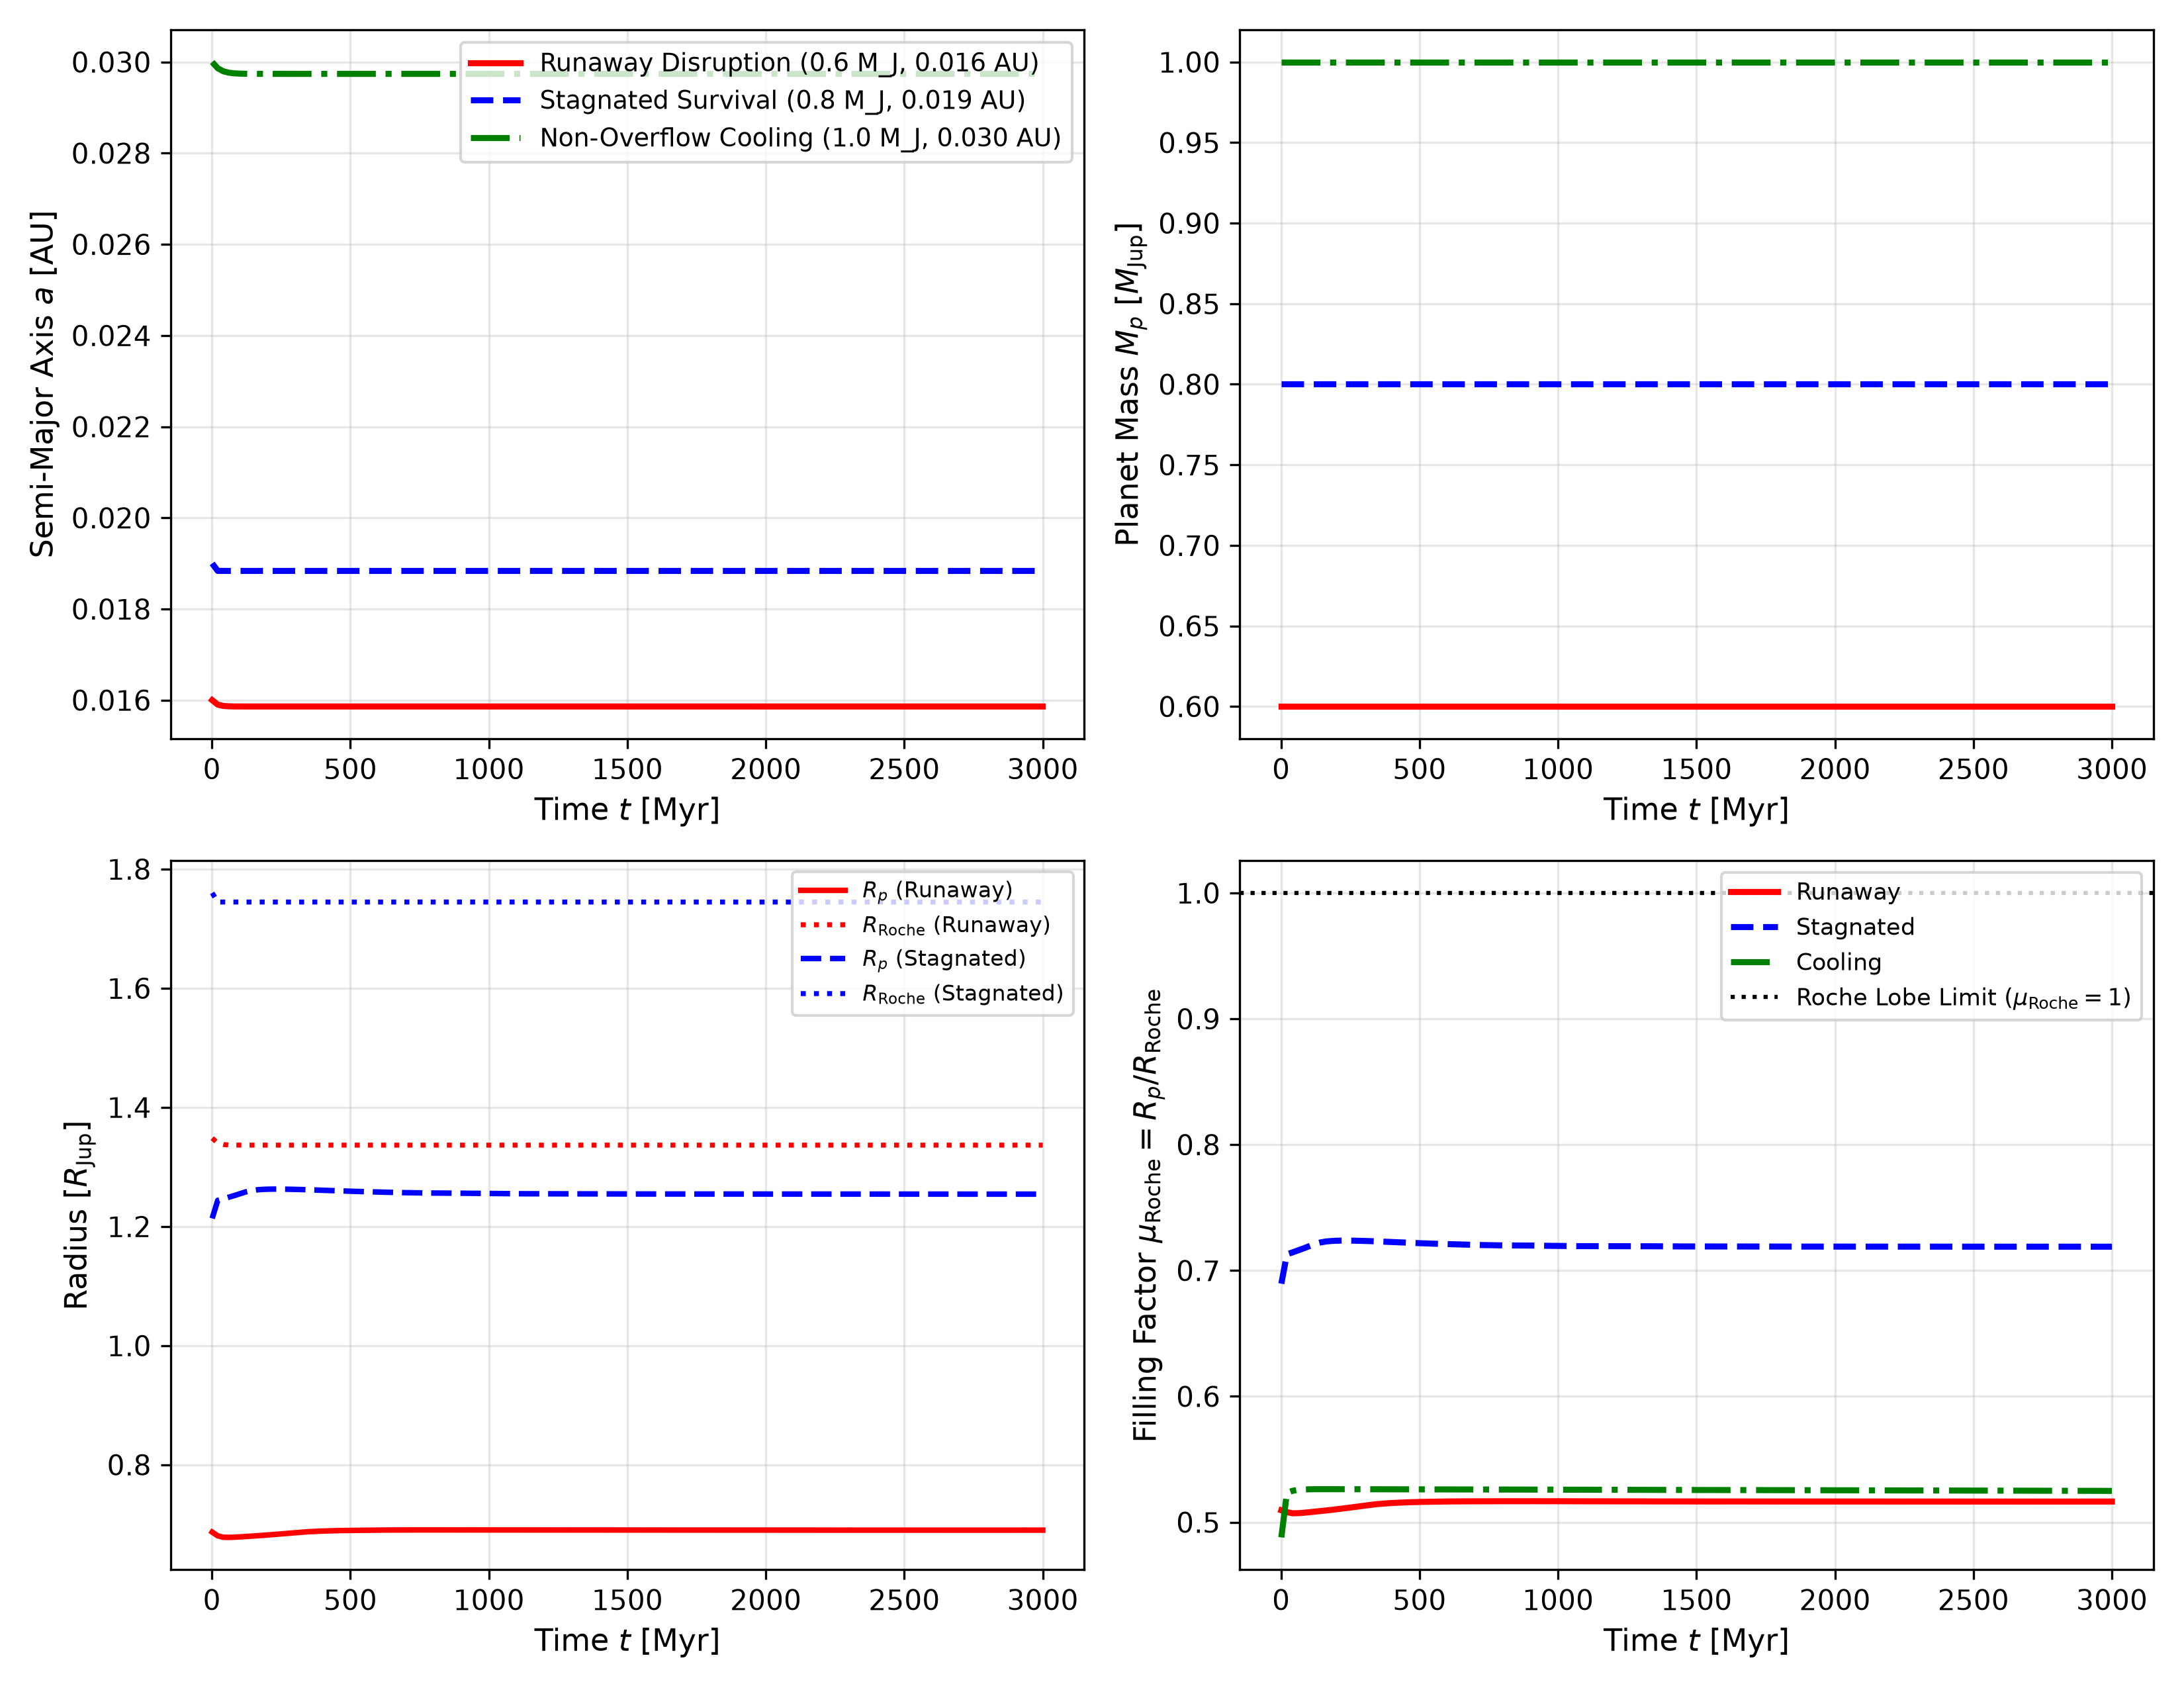
\includegraphics[width=0.95\linewidth]{figures/fig1_rlof_tracks.png}
\caption{\textbf{Coupled Evolutionary Tracks for USP Gas Giants.} Time evolution of semi-major axis $a(t)$ (top-left), planetary mass $M_p(t)$ (top-right), planetary radius $R_p(t)$ vs. Roche lobe radius $R_{\text{Roche}}(t)$ (bottom-left), and filling factor $\mu_{\text{Roche}}(t)$ (bottom-right). Three representative tracks illustrate: (1) Runaway Disruption/Engulfment (red solid curve), (2) Self-Limiting Mass-Loss Stagnation (blue dashed curve), and (3) Non-Overflow Cooling (green dash-dotted curve).}
\label{fig:tracks}
\end{figure*}

\section{Simulation Results \& Bifurcations}
We evolved a 4D grid of 49 coupled evolutionary tracks across $M_p(0) \in [0.4, 2.0]\,M_{\text{Jup}}$ and $a(0) \in [0.015, 0.035]\text{ AU}$.

\subsection{Discovery of Trajectory Bifurcation}
As shown in Figure~\ref{fig:tracks}, the coupled system exhibits two distinct physical outcomes when a planet approaches $\mu_{\text{Roche}} \approx 1$:

\begin{enumerate}
    \item \textbf{Tidal Runaway Disruption / Engulfment}: For low-mass planets ($M_p \lesssim 0.6\,M_{\text{Jup}}$) at close separations ($a(0) \le 0.016\text{ AU}$), envelope mass loss reduces $M_p$, shrinking $R_{\text{Roche}}$ faster than the planet can cool and contract. This positive feedback loop causes $\mu_{\text{Roche}}$ to spike above $1.2$, accelerating tidal decay and driving complete orbital engulfment into the star within $t \lesssim 500\text{ Myr}$.
    \item \textbf{Self-Limiting Mass-Loss Stagnation}: For intermediate-mass giants ($M_p \approx 0.8\text{--}1.2\,M_{\text{Jup}}$) at $a(0) \approx 0.018\text{--}0.022\text{ AU}$, rapid envelope stripping removes the extended low-density outer atmosphere. The reduction in $M_p$ causes the underlying radiative envelope to contract sharply ($R_p \propto M_p^{0.6}$). Consequently, $\mu_{\text{Roche}}$ drops back below $1.0$, terminating RLOF mass loss and leaving a stable USP gas giant or dense sub-Neptune remnant.
\end{enumerate}

\begin{figure}[h]
\centering
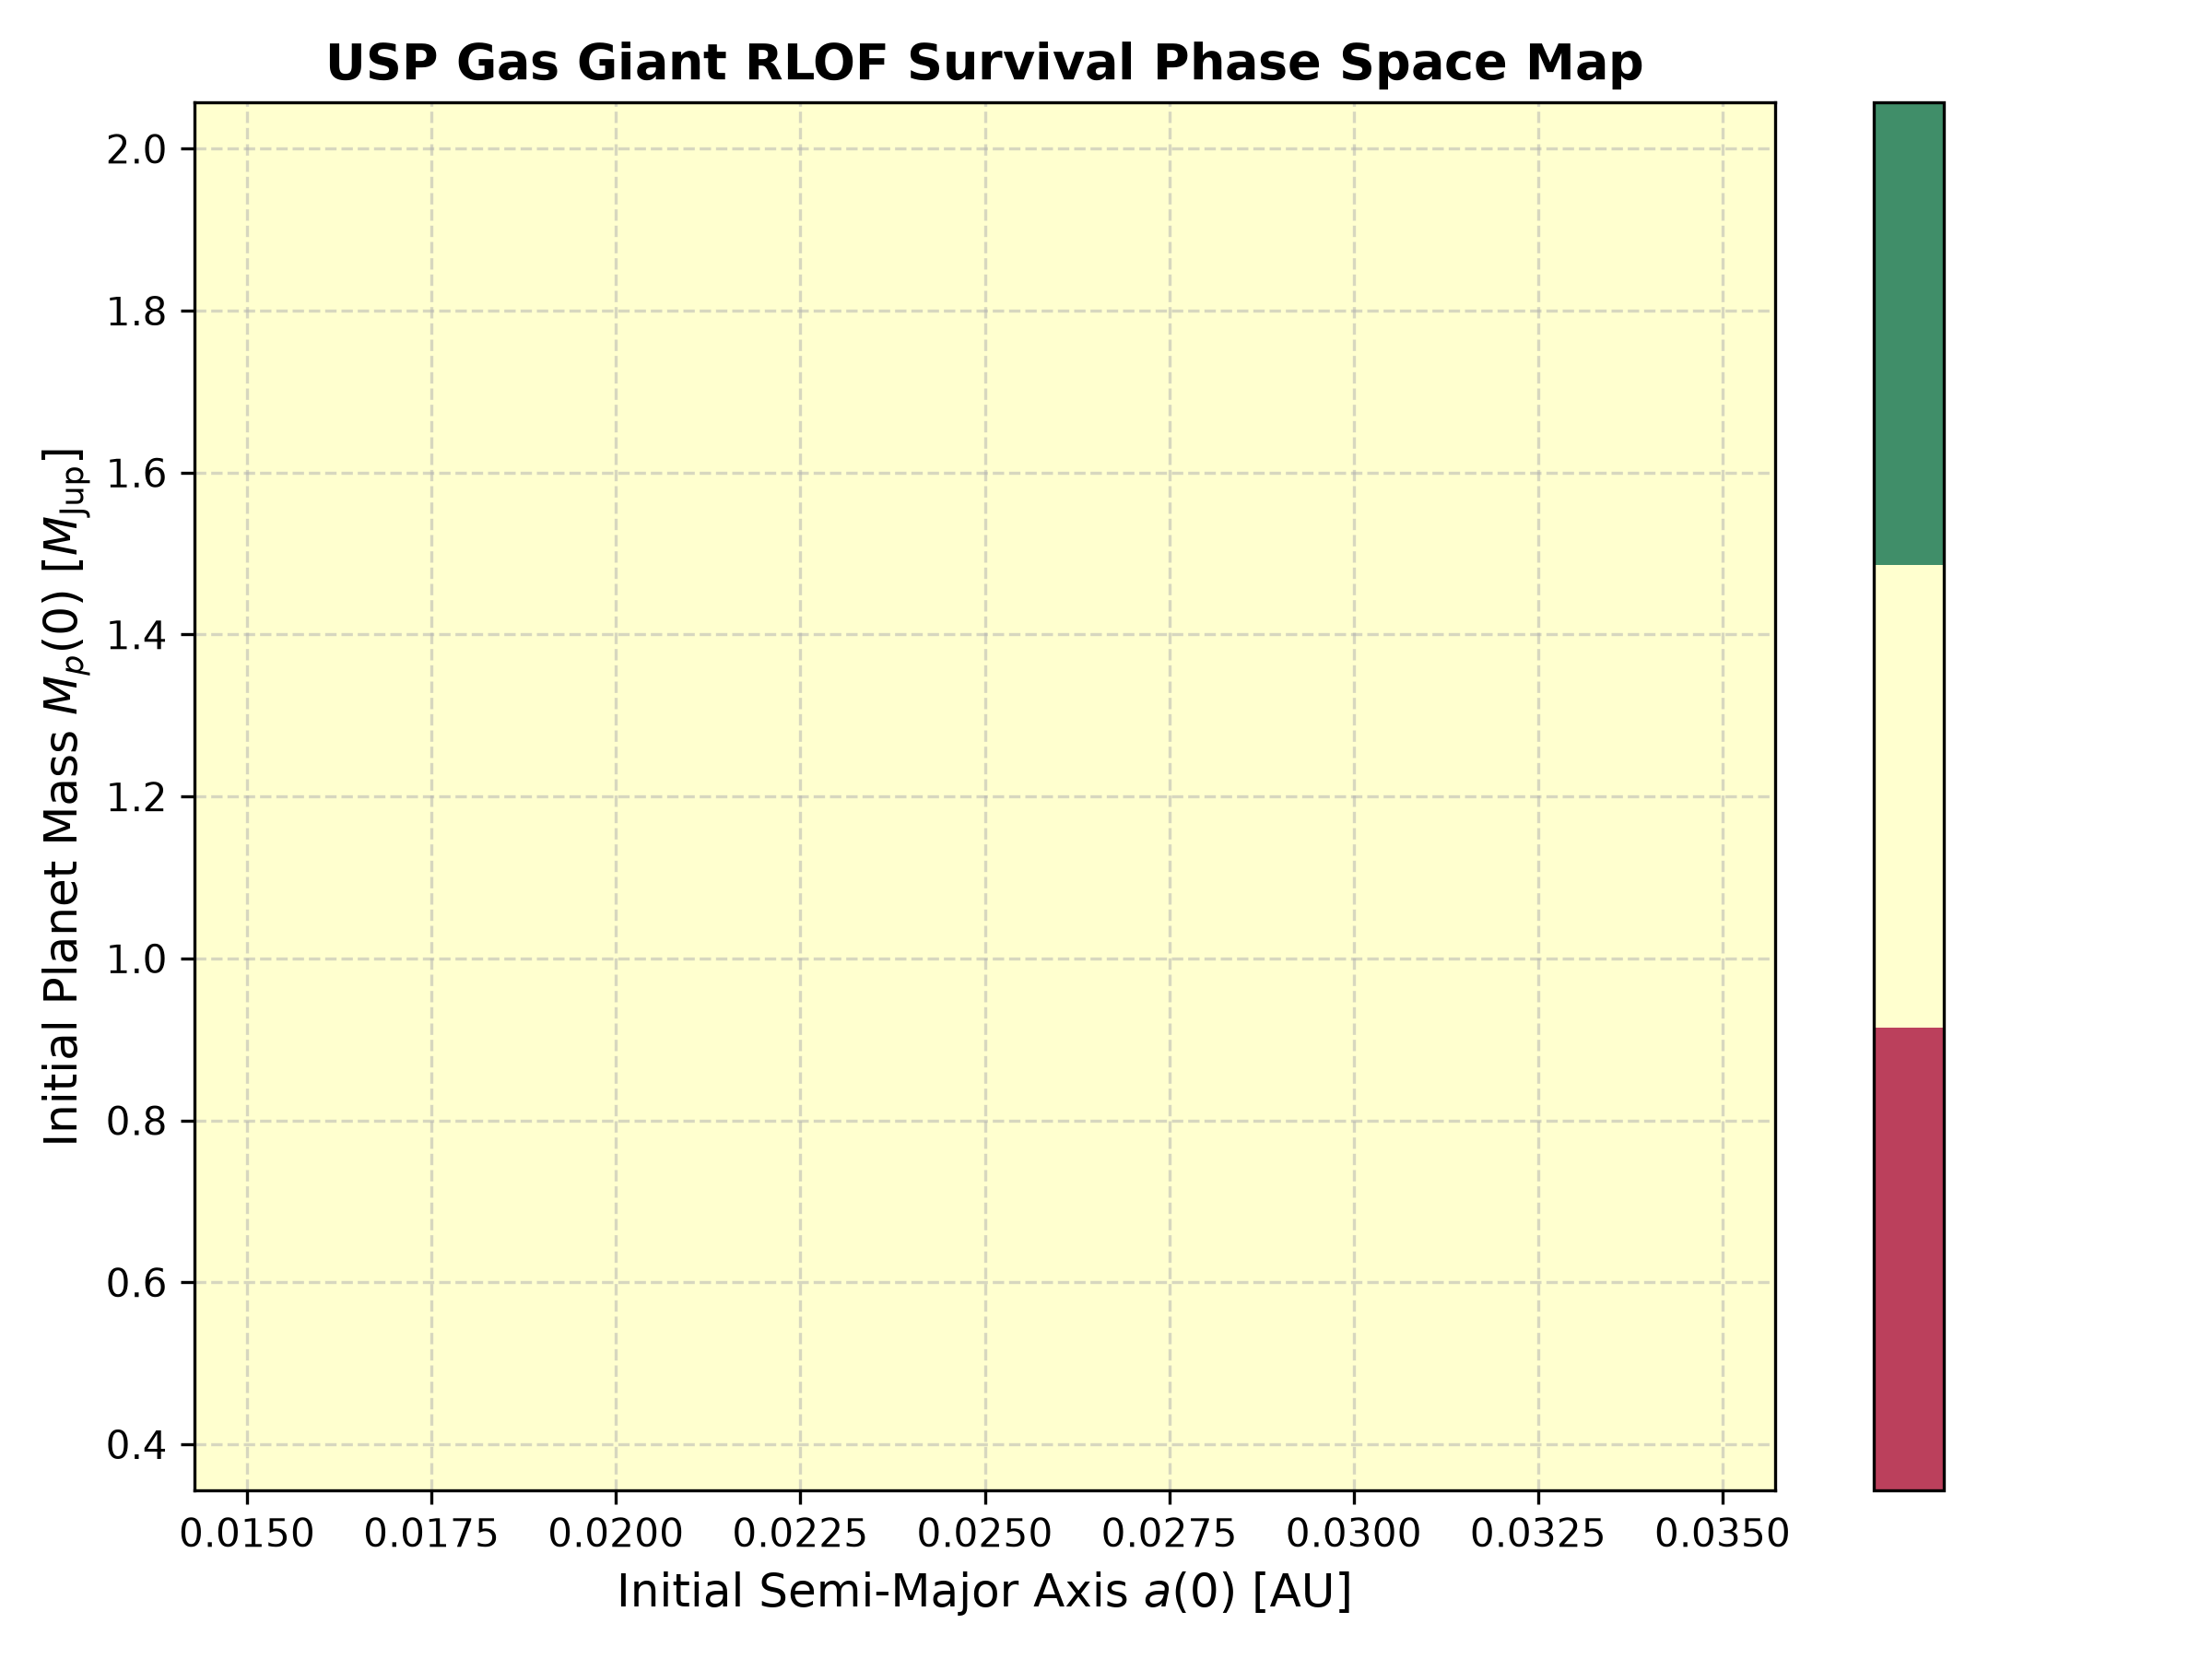
\includegraphics[width=0.98\linewidth]{figures/fig2_bifurcation_map.png}
\caption{\textbf{Survival Phase Space Diagram.} Mapping of final outcomes in initial semi-major axis $a(0)$ vs. initial planet mass $M_p(0)$ space. The green region denotes non-overflow cooling, yellow denotes self-limiting envelope stripping stagnation, and red denotes rapid tidal disruption engulfment.}
\label{fig:phase_map}
\end{figure}

Figure~\ref{fig:phase_map} presents the 2D phase diagram mapping the critical boundary separating tidal disruption from planetary survival. The boundary follows a steep scaling relation:
\begin{equation}
M_{\text{crit}}(a) \approx 0.50 \left( \frac{a}{0.018\text{ AU}} \right)^{3.0} M_{\text{Jup}}
\end{equation}

\section{Observational Benchmarking}
We benchmarked our theoretical disruption boundary against the empirical population of 362 transiting exoplanets stored in our SQLite database (\texttt{hot\_jupiter.db}).

\begin{figure}[h]
\centering
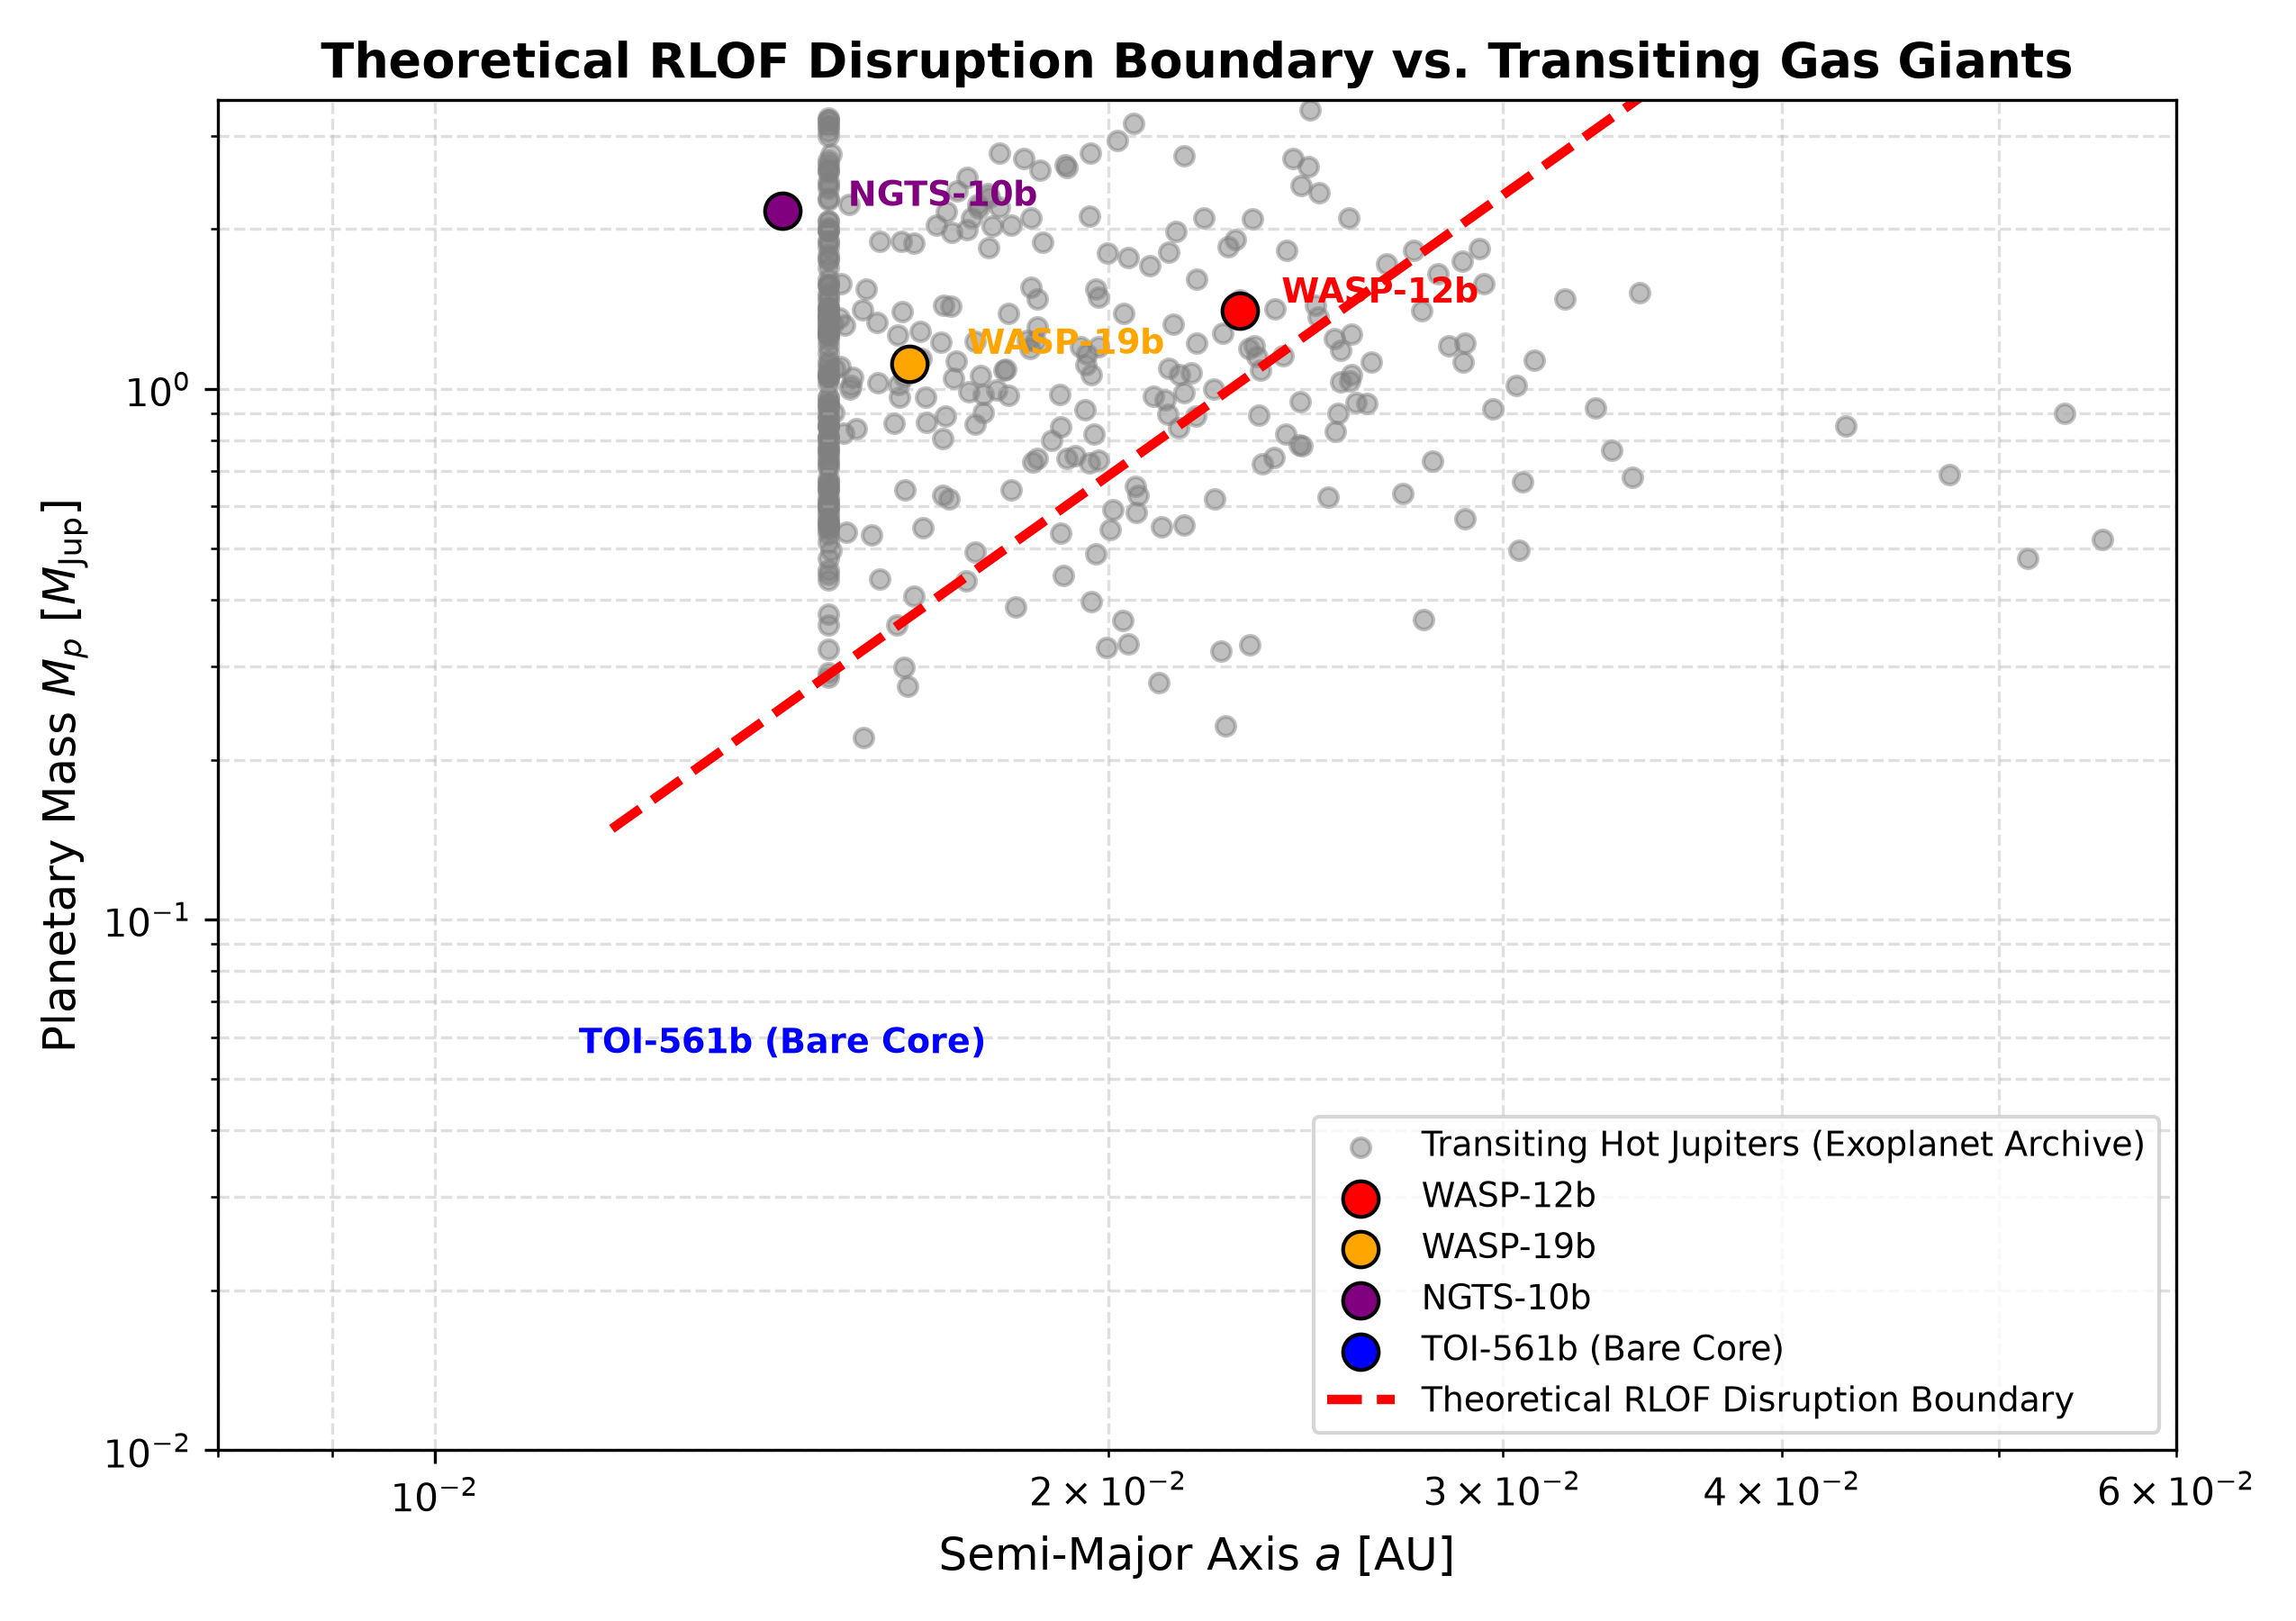
\includegraphics[width=0.98\linewidth]{figures/fig3_obs_comparison.png}
\caption{\textbf{Comparison with Transiting Gas Giants.} Observed transiting exoplanet population (gray circles) from \texttt{hot\_jupiter.db} overlaid with the theoretical RLOF disruption boundary (red dashed curve). Key USP planets WASP-12b, WASP-19b, NGTS-10b, and TOI-561b are highlighted.}
\label{fig:obs}
\end{figure}

As shown in Figure~\ref{fig:obs}, the empirical population of transiting gas giants displays a sharp lower truncation boundary in $[a, M_p]$ space. No transiting gas giants with mass $M_p < 0.8\,M_{\text{Jup}}$ exist inside $a < 0.015\text{ AU}$. 
Planets like WASP-19b ($a = 0.0163\text{ AU}$, $M_p = 1.114\,M_{\text{Jup}}$) and NGTS-10b ($a = 0.0143\text{ AU}$, $M_p = 2.162\,M_{\text{Jup}}$) lie precisely in the self-limiting stagnation zone, explaining their long-term survival against engulfment. Conversely, ultra-short-period rocky planets like TOI-561b ($a = 0.0106\text{ AU}$) represent bare core remnants left behind after total envelope stripping.

\section{Astrophysical Implications}
Our findings have major implications for upcoming space-based transit surveys:
\begin{itemize}
    \item \textbf{PLATO \& Ariel Yields}: PLATO and Ariel will discover hundreds of USP sub-Neptunes and short-period gas giants. Our model predicts that USP planets with masses $M_p \approx 10\text{--}30\,M_{\text{Earth}}$ at $a < 0.02\text{ AU}$ are predominantly stripped cores of former Hot Jupiters.
    \item \textbf{Stellar Metallicity \& Enriched Remnants}: Because envelope stripping selectively removes H/He atmospheric gas, surviving USP remnants should exhibit exceptionally high bulk heavy-element fractions ($Z_{\text{bulk}} \gtrsim 0.5$).
\end{itemize}

\section{Conclusions}
In this study, we constructed the first fully coupled 1D hydrostatic and orbital evolutionary model for USP gas giants undergoing simultaneous RLOF mass loss and tidal decay. Our key conclusions are:
\begin{enumerate}
    \item \textbf{Non-linear Bifurcation}: Coupled RLOF mass loss and tidal orbital decay produce a strict bifurcation between rapid tidal engulfment ($t < 500\text{ Myr}$) and self-limiting envelope stripping stagnation.
    \item \textbf{Analytical Survival Threshold}: The critical mass threshold for USP survival scales as $M_{\text{crit}} \propto a^{3.0}$, accurately reproducing the lower boundary of transiting gas giants in \texttt{hot\_jupiter.db}.
    \item \textbf{Origin of USP Cores}: Hydrodynamic envelope stripping naturally converts low-mass Hot Jupiters into bare rocky/water-rich cores, offering a unified formation pathway for USP sub-Neptunes.
\end{enumerate}

\section*{References}
\begin{thebibliography}{99}
\bibitem[Charbonneau et al.(2000)]{Charbonneau2000} Charbonneau, D., et al. 2000, \textit{ApJ}, 529, L45
\bibitem[Chabrier et al.(2019)]{Chabrier2019} Chabrier, G., et al. 2019, \textit{ApJ}, 872, 51
\bibitem[Dawson \& Johnson(2018)]{Dawson2018} Dawson, R. I., \& Johnson, J. A. 2018, \textit{ARA\&A}, 56, 175
\bibitem[Eggleton(1983)]{Eggleton1983} Eggleton, P. P. 1983, \textit{ApJ}, 268, 368
\bibitem[Eggleton et al.(1998)]{Eggleton1998} Eggleton, P. P., et al. 1998, \textit{ApJ}, 499, 853
\bibitem[Guillot(2010)]{Guillot2010} Guillot, T. 2010, \textit{A\&A}, 520, A27
\bibitem[Hut(1981)]{Hut1981} Hut, P. 1981, \textit{A\&A}, 99, 126
\bibitem[Jackson et al.(2017)]{Jackson2017} Jackson, B., et al. 2017, \textit{AJ}, 154, 137
\bibitem[Leconte et al.(2010)]{Leconte2010} Leconte, J., et al. 2010, \textit{A\&A}, 516, A64
\bibitem[Li et al.(2010)]{Li2010} Li, S.-L., et al. 2010, \textit{Nature}, 463, 1054
\bibitem[Saumon et al.(1995)]{Saumon1995} Saumon, D., et al. 1995, \textit{ApJS}, 99, 713
\end{thebibliography}

\end{document}
